\documentclass[a4paper,11pt]{article}
%\pdfoutput=1 % if your are submitting a pdflatex (i.e. if you have
%             % images in pdf, png or jpg format)

\usepackage{jcappub} % for details on the use of the package, please
                     % see the JCAP-author-manual
\usepackage{siunitx}
\usepackage[T1]{fontenc} % if needed
\usepackage{subcaption}


\title{\boldmath A title with some math: $x=1$}


%% %simple case: 2 authors, same institution
%% \author{A. Uthor}
%% \author{and A. Nother Author}
%% \affiliation{Institution,\\Address, Country}

\author{Jack Dinsmore}
\author{and Tracy Slatyer}
\affiliation{Massachusetts Institute of Technology \\Cambridge, MA, USA}

% e-mail addresses: one for each author, in the same order as the authors
\emailAdd{jtdinsmo@mit.edu}
\emailAdd{tslater@mit.edu}

\newcommand{\parens}[1]{\left(#1\right)}
\newcommand{\brackets}[1]{\left[#1\right]}
\newcommand{\expp}[1]{\exp \parens{#1}}
\newcommand{\fraci}[2]{#1 / #2}
\newcommand{\comment}[1]{\emph{\color{red}{#1}}}

\DeclareSIUnit\erg{erg}
\DeclareSIUnit\parsec{pc}
\DeclareSIUnit\photon{photon}



\abstract{Abstract...}



\begin{document}
\maketitle
\flushbottom



\section{Introduction}



\section{Methods \& Datasets}
\subsection{GCE Spacial distribution}
We model the spacial distribution of MSPs in the GC with an NFW squared profile, to match with empirical data. The number density of an NFW profile is spherically symmetric, with radial density profile
\label{sec:spacial-distro}
\begin{equation}
    \rho_\text{NFW}(r) \propto \parens{\frac{r}{r_s}}^{-\gamma}\parens{1 + \frac{r}{r_s}}^{-3-\gamma}
    \label{eqn:nfw}
\end{equation}
where $\gamma = 1.2$ and $r_s = \SI{20}{\kilo\parsec}$ for this work. Other sources occasionally use $\gamma = 1$.

We allow this NFW distribution to extend over a region of interest (ROI) extending within $|\ell| < 20^\circ$ and $2^\circ < |b| < 20^\circ$, where we have cut out the Galactic disk. We also restrict the luminosity of the GCE to within $\SI{0.1}{\giga\electronvolt} < E_\gamma < \SI{100}{\giga\electronvolt}$. Both these ranges are slightly on the larger side of those commonly used in literature.


\subsection{Observables}
\label{sec:observables}
To fit the luminosity functions described in section \ref{sec:lum-funcs}, we will use three observables: the total flux of the GCE $F_\text{GCE}$, the ratio of the total flux to the flux visible from point sources resolved by \textit{Fermi} $R_\text{r}$, and the number of resolved point sources $N_\text{r}$. The first observable, $F_\text{GCE}$, is described in section \ref{sec:total-lum}, but we describe the other two observables in this section.

$N_\text{r}$ and $R_\text{r}$ have been studied by \comment{Some technical name for the Fermilab team.} \cite{Zhong:2019ycb}. The authors performed a template fit to data from Fermi-LAT to isolate spacial peaks in flux, finding 110 \comment{(I got 110; their paper says 107)} peaks within 0.3$^\circ$ of a source in the 4FGL catalog within the region of interest \cite{Abdollahi_2020}. Of these 110 sources, they exclude all that are listed in the 4FGL catalog as not associated with pulsars. Of those that are known to be pulsars, they exclude all whose positions are known not to be within 2 kpc of the GC via the ATNF Pulsar Catalog \cite{Hobbs04}. This leaves 47 point sources in the 4FGL catalog whose origins are either known to be pulsars in the GC or are unknown. We will therefore set $N_\text{r} = 47$ for this paper. If the allowed distance between a flux peak and a 4FGL source is extended from 0.3$^\circ$ to $0.55^\circ$, five more sources are added. Together, the 47 sources are responsible for $R_\text{r}=0.2$ of the total GCE flux. \comment{Shouldn't I actually redo this addition given the fact that I'm now not using the same GCE flux as Fermilab?} These 47+5 sources used here are displayed in figure \ref{fig:47-sources}.

\begin{figure}
    \centering
    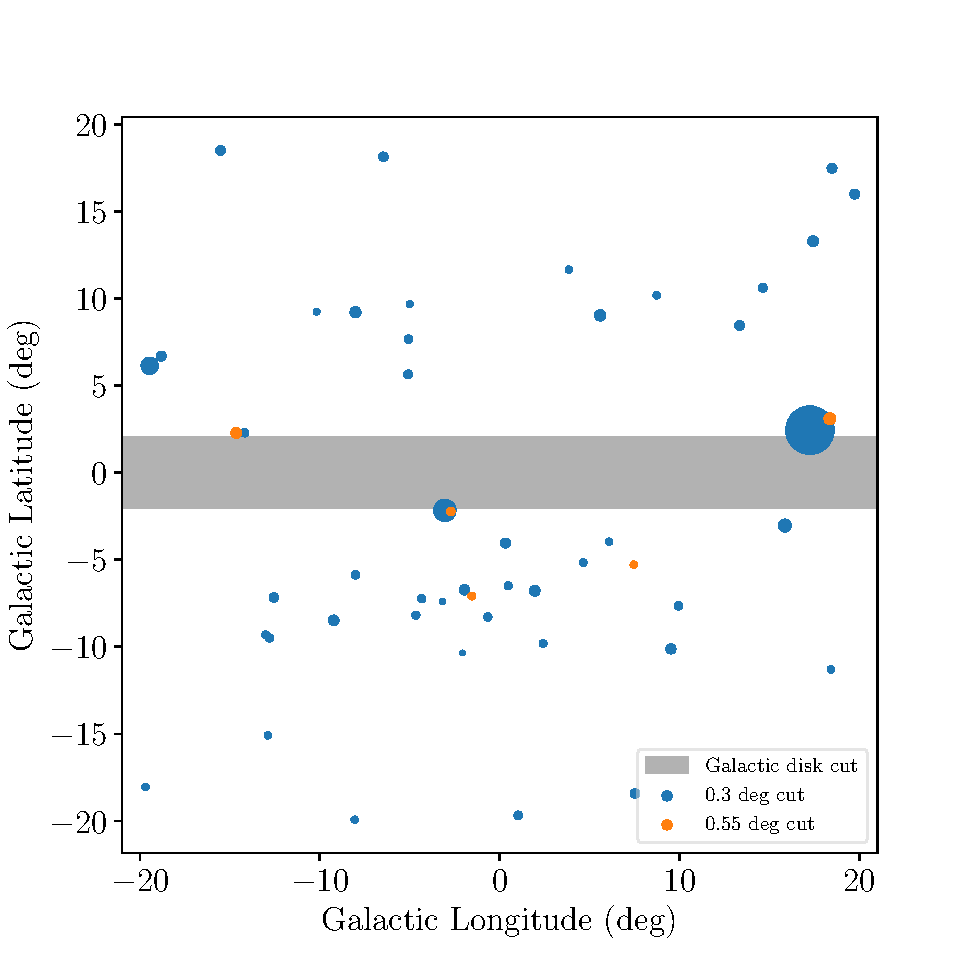
\includegraphics[width=0.5\textwidth]{figs/point-source-positions.pdf}
    \caption{The 47 point sources within $0.3^\circ$ of a 4FGL source. Also shown are the 5 sourecs added by extending to $0.55^\circ$ separation. The sources are scaled by luminosity in radius. The gray band represents the $|b| \leq 2^\circ$ cut made around the galactic disk.}
    \label{fig:47-sources}
\end{figure}

It is important to note that the above values for $N_\text{r}$ and $R_\text{r}$ define an allowed region, which includes populations with lower $N_\text{r}$ and $R_\text{r}$, because some of the unknown sources might not be pulsars.



We will also discuss a third feature of a potential MSP population in the GC: the total number of MSPs $N_\text{GCE}$, resolved or unresolved. This number is not measurable, but serves as a useful reference to gauge the physicality of any population of MSPs. \comment{Mention that it's expected to be around 40,000.}


\subsection{Total GCE Luminosity}
\label{sec:total-lum}
Since an estimate of the total flux of the GCE is necessary for our data, we extract the total flux from several previous analyses of spectra using the following three methods and compare them. The spectral analyses we study here are refs. \cite{Zhong:2019ycb, Calore:2014xka, DiMauro:2021raz, Abazajian:2014fta, Gordon, Ajello}. Each reference reports the total flux $F_\gamma(E)$ observed in an energy bin centered on $E$. The spectra from these sources are reported in figure \ref{fig:all-spectra}
\begin{figure}
    \centering
    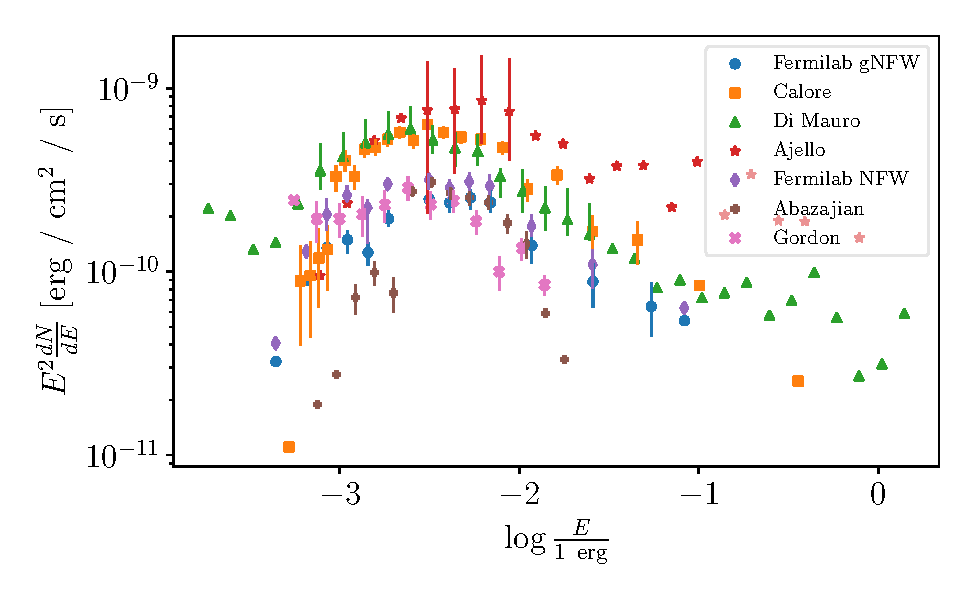
\includegraphics[width=0.5\textwidth]{figs/all-spectra.pdf}
    \caption{Spectra from seven analyses of the GCE, using different background models, shown with error bars when reported.}
    \label{fig:all-spectra}
\end{figure}

\comment{Describe the sources: what's similar between them, what's different.}

We use compare three methods of extracting the total GCE flux from these analyses.
The first method is direct numerical integration of the spectra provided by each source. This method is most sensitive to the data measured by \textit{Fermi} and does not attempt to abstract over it with a smooth function.

However, numerical integration cannot account for the spectrum lying outside of \textit{Fermi}'s spectrum of sensitivity, and it may be oversensitive to experimental error. Therefore, we also consider a broken law fit to the data, of the same form as the NPTF luminosity function: eq. \ref{eqn:nptf}. It has four parameters: a constant of proportionality, the turnover flux $F_\text{b}$, and the slopes above and below the turnover flux $n_2$ and $n_1$. This function can then be analytically integrated over all flux values to get the total flux of the GCE. Many of the analyses cited above only report error bars on some points, because error bars on the other points are too large. We therefore fit only to the points with error bars reported. \comment{Mention the specific range fitted over}.

Unfortunately, for some analyses, the number of points reported with error bars is only slightly larger than the number of parameters of the broken power law function. To ensure that the fit result is less prone to statistical deviations of a small number of points, we use a third method in addition to the above two. Ref. \cite{Calore:2014xka} provides their fit parameters for their GCE flux spectral data: $F_\text{b} = $. $n_1 = -1.42$, $n_2 = 2.63$. \comment{Check for sign errors in the original. Also get the flux they provide.}. The third fitting method is to fix these three broken power law parameters at these values and allow only the overall normalization to vary. An example of all three of these fitting methods applied to reference \cite{DiMauro:2021raz} and shown in figure \ref{fig:di-mauro-example}.

\begin{figure}
    \centering
    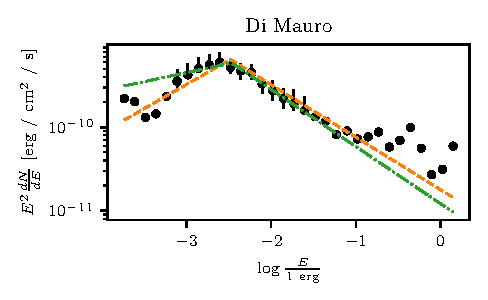
\includegraphics[width=0.5\textwidth]{figs/di-mauro-example.pdf}
    \caption{Spectrum produced by di Mauro in ref. \cite{DiMauro:2021raz}, with the two broken power law models fitted and shown.}
    \label{fig:di-mauro-example}
\end{figure}

In practice, the three fitting methods yield very similar results for a single analysis. However, the values provided by different analyses vary greatly. For this study, we use the value obtained from di Mauro's analysis because it occupies a position near the middle of the distribution of GCE luminosities and is a recent study. We choose the value obtained by numerical integration, which is $F_\text{GCE} = \SI{1.295e-9}{\erg\per\centi\meter\squared\per\second}$.

\comment{Discuss how rescaling of the ROI was done}

\begin{figure}
    \centering
    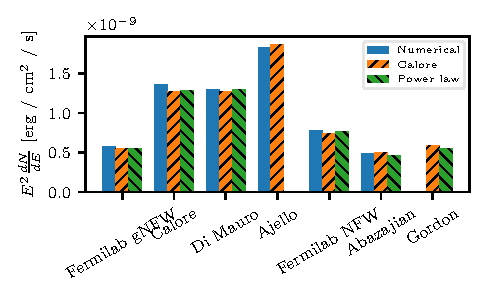
\includegraphics[width=0.5\textwidth]{figs/total-flux-bars.pdf}
    \caption{Total flux of the GCE as determined by the three integration methods discussed. \comment{Here I would discuss why Ajello doesn't have a value for the power law case if this is still true once I have the original source}.}
    \label{fig:total-flux-bars}
\end{figure}


\comment{Just double check that I normalized the power law correctly in parse\_spectrum.py.}

\subsection{Luminosity Functions}
\label{sec:lum-funcs}
Previous work has interpreted this MSP model. Ref. \cite{Zhong:2019ycb} has proposed an exponentially damped power law luminosity function
\begin{equation}
    P_\text{Power law}(L) = L^{-\alpha} \expp{-\frac{L}{L_\text{max}}}\brackets{\Gamma\parens{1-\alpha, \frac{L_\text{min}}{L_\text{max}}}L_\text{max}^{1-\alpha}}^{-1}.
    \label{eqn:power-law}
\end{equation}
The function has been normalized so that $P_\text{Power law}(L)$ represents the probability that a given MSP has luminosity $L$. This luminosity function restricts the range of luminosities to $[L_\text{min}, \infty)$, where $L_\text{min}$, $L_\text{max}$, and $\alpha$ are free parameters. \comment{The following should probably be moved to the introduction, where Fermilab's research is described.} This reference found that $(\SI{1e29}{\erg\per\second}, \SI{1e35}{\erg\per\second}, 1.94)$ is required reproduced observations. They find that this model admits three million MSPs in the GCE, which differs from estimates based on the physical properties of observed MSPs that estimate the number of MSPs at the Galactic center at the order of 40,000 \cite{citation_needed}.

Ref. \cite{osti_1305131} proposes a power law luminosity function of
\begin{equation}
    P_\text{Log normal}(L)= \frac{\log_{10} e}{\sigma \sqrt{2\pi} L}\expp{-\frac{\parens{\log_{10} L - \log_{10} L_0}^2}{2\sigma^2}},
    \label{eqn:log-normal}
\end{equation}
where $L_0$ and $\sigma$ are free parameters. The ref. fits this model to data from globular cluster (GCL) data, yielding values $L_0 = \SI{8.8e33}{\erg\per\second}$ and $\sigma=0.62$. It predicts thousands of MSPs to occupy the GCE if the entire excess is to be explained by MSPs.

Ref. \cite{Ploeg:2020jeh} proposes several more intricate luminosity functions, derived from a model of the pulsars themselves. They find that the same model may be used for resolved, globular cluster MSPs in the Galactic disk and unresolved MSPs at the Galactic center. We use their luminosity function generated for the galactic disk. It closely resembles a log normal luminosity function as in equation \ref{eqn:log-normal}, where $L_0 = \SI{1.61e+32}{\erg\per\second}$ and $\sigma=0.700$.

Another study by Gautam et al. analyzes the possibility that the hypothetical MSP population in the GCE is generated not by the Low Mass X-Ray Binary formation, but by Accretion Induced Collapse \cite{Gautam:2021wqn}. \comment{To distinguish between this, a definition of these two collapse methods, along with models other than an MSP model, should be put in the introduction. Mention the fact that the MSPs in the GCE would have to look different from that in the disk.} Their binary system model yields a numerical luminosity function for MSPs in the GC, reported as a function of flux. Converting to luminosity in the manner described in appendix \ref{app:lum-to-flux}, we find that a log normal distribution fits their function well, with $L_0 = \SI{3.92e+32}{\erg\per\second}$ and $\sigma = 0.937$. We call this model the AIC Log normal model.

Finally, ref. \cite{Lee:2015fea} proposes a broken-power law luminosity function of
\begin{equation}
    P_\text{NPTF}(L) = \parens{\frac{\parens{1-n_1}\parens{1-n_2}}{L_b \parens{n_1 - n_2}}}\begin{cases}
        \parens{\fraci{L}{L_\text{b}}}^{-n_{1}} & L < L_{b} \\
        \parens{\fraci{L}{L_\text{b}}}^{-n_{2}} & L > L_b
    \end{cases}
    \label{eqn:nptf}
\end{equation}
where the free parameters  $n_1$, $n_2$, and $L_b$ were found via a Non-Poissonian Template Fitting model (NPTF) to be $(18.2, -0.66, \SI{8.66e+33}{\erg\per\second})$ for an NFW-squared-distributed population of MSPs named NFW PS. The paper proposes a second luminosity function named Disk PS with parameters $(17.5, 1.4, \SI{3.34e+35}{\erg\per\second})$, which is unnormalizable except when a minimum luminosity of pulsars $L_\text{min}$ is introduced. \comment{I will want to remove the unnormalizable one. When should I do it?} The luminosity-valued parameters were originally given as fluxes in $\SI{}{\photon \per \centi\meter\squared \per \second}$. The photon energy was calculated via appendix \ref{app:photon-energy} and the flux converted to luminosity via appendix \ref{app:lum-to-flux}.

We set $L_\text{min}=\SI{1e29}{\erg\per\second}$, which is the same minimum pulsar luminosity used by ref. \cite{Zhong:2019ycb}. The turnover luminosity $L_\text{b}$ was given as a photon flux value in units of photons per centimeter squared per second; the process used to convert from photon flux to luminosity is detailed in the methods section.

All the above-mentioned luminosity functions are shown in figure \ref{fig:lum-funcs}.

\begin{figure}
    \centering
    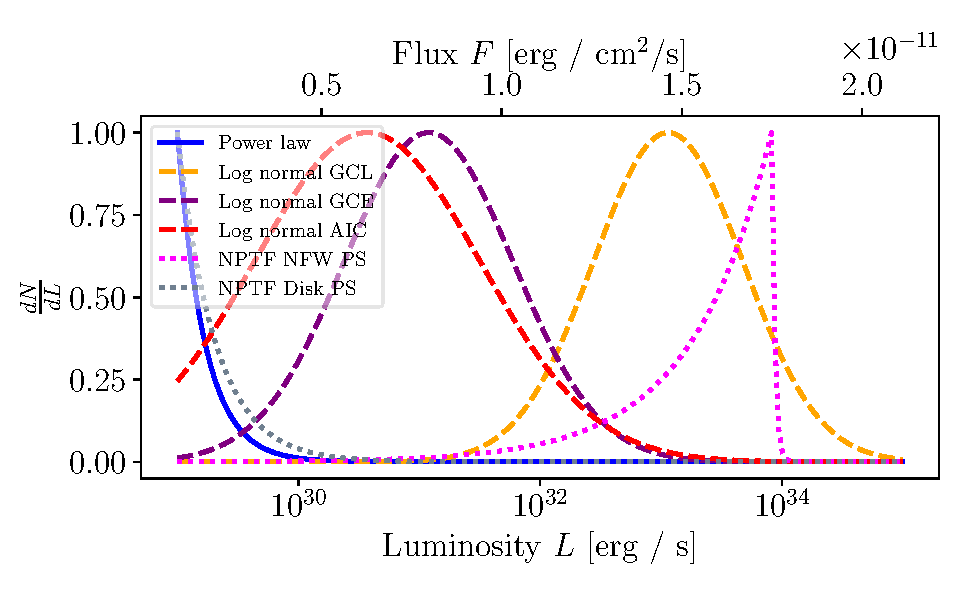
\includegraphics[width=0.49\textwidth]{figs/lum-funcs.pdf}
    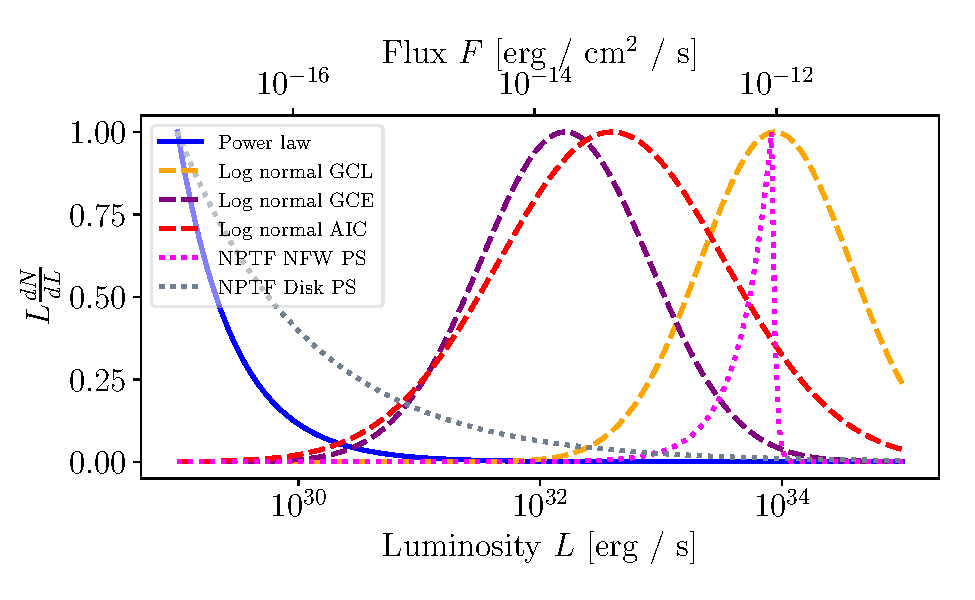
\includegraphics[width=0.49\textwidth]{figs/l-lum-funcs.pdf}
    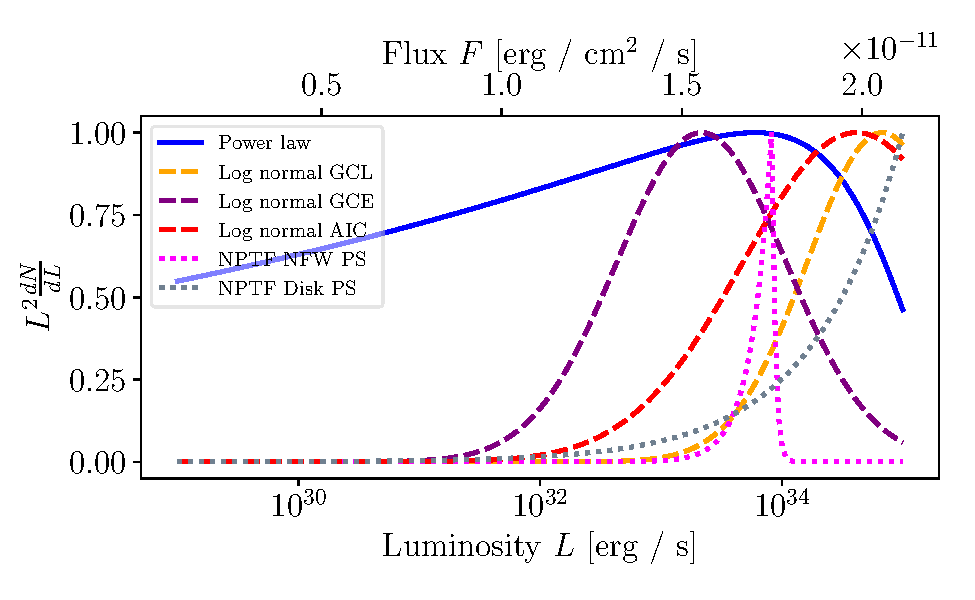
\includegraphics[width=0.49\textwidth]{figs/l2-lum-funcs.pdf}
    \caption{\textit{Left:} Power law, GCL log normal, GCE log normal, and NPTF luminosity functions for MSPs in the GCE, vertically rescaled. \textit{Right:} Same plot as \textit{left} but weighted by luminosity. \textit{Bottom:} Same plot as above two but weighted by luminosity squared.}
    \label{fig:lum-funcs}
\end{figure}


\subsection{Sensitivity Models}
\label{sec:sensitivity}
The \textit{Fermi} telescope does not detect every pulsar in the GC; background emission obscures dimmer pulsars, and statistical effects cause some bright sources to be unresolved. We make use of three sensitivity models to model these factors.

The first, and simplest, is a step function luminosity model. It asserts that all point sources with $L>L_\text{th}$ are resolved, and none with $L<L_{\text{th}}$. Here, $L_\text{th} = \SI{e34}{\erg\per\second}$. This sensitivity model is the one used by ref. \cite{Zhong:2019ycb} to obtain the parameters of the power law luminosity function described in the paragraph after eq. \ref{eqn:power-law}. The four properties we intend to measure are then given by
\begin{equation}
    \begin{split}
        L_\text{GCE} &= N_\text{GCE}\int_{L_\text{min}}^\infty L P(L) dL \,, \qquad
        L_\text{r} = N_\text{GCE}\int_{L_\text{th}}^\infty L P(L) dL \,, \\
        N_\text{r} &= N_\text{GCE}\int_{L_\text{th}}^\infty P(L) dL \,,
        \label{eqn:observables-sens-1}
    \end{split}
\end{equation}
where $N_\text{GCE}$ is a normalization constant, fixed by requiring that $L_\text{GCE}$ reproduces the flux $F_\text{GCE}$ observed. The conversion between $L_\text{GCE}$ and $F_\text{GCE}$ is outlined in appendix \ref{app:lum-to-flux}.

The second sensitivity model acknowledges the effect of background flux on resolvability and uses a position-dependent flux threshold $F_\text{th}(b, l)$ published by the \textit{Fermi} team \cite{Fermi-LAT:2019yla, Ballet:2020hze} (figure \ref{fig:sensitivity}). \comment{Here, I could talk about how to convert between flux and luminosity and then use the mean of this map to assess how accurate 1e34 ergs/s actually is.}. To calculate the four properties of GC MSP populations, we use
\begin{equation}
    \begin{split}
        F_\text{GCE} &= \int_\Omega d\Omega \int_0^\infty s^2 ds A \rho_{NFW}^2(r)\int_{L_\text{min}}^\infty dL \frac{L}{4\pi s^2}P(L)\,, \\
        N_\text{GCE} &= \int_\Omega d\Omega \int_0^\infty s^2 ds A \rho_{NFW}^2(r)\,, \\
        F_\text{r} &= \int_\Omega d\Omega \int_0^\infty s^2 ds A \rho_{NFW}^2(r)\int_{4\pi s^2F_\text{th}(b,\ell)}^\infty dL \frac{L}{4\pi s^2}P(L)\,, \\
        N_\text{r} &= \int_\Omega d\Omega \int_0^\infty s^2 ds A \rho_{NFW}^2(r)\int_{4\pi s^2F_\text{th}(b,\ell)}^\infty dL P(L) \,. \\
        \label{eqn:observables-sens-2}
    \end{split}
\end{equation}
Here, $\Omega$ represents the $20^\circ \times 20^\circ$ region of interest with $|b| < 2^\circ$ cut out, and $A$ is the coefficient of equation \ref{eqn:nfw}, fixed by forcing $F_\text{GCE}$ to equal the observed value. In equation \ref{eqn:observables-sens-2} represents the distance to the galactic center from the point of integration, and is determined by the law of cosines:
$r^2 = s^2 + r_c^2 - 2r_c s \cos \ell$.

\begin{figure}
    \centering
    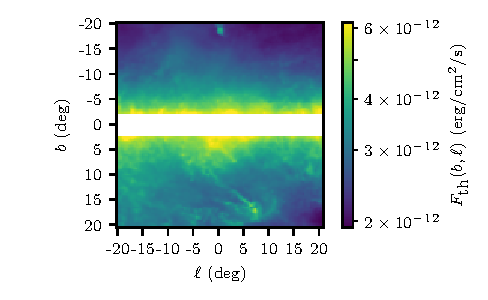
\includegraphics[width=0.7\textwidth]{figs/sensitivity-map.pdf}
    \caption{Position-dependent flux thresholds required to resolve an MSP, published by refs. \cite{Fermi-LAT:2019yla, Ballet:2020hze}. \comment{Maybe I shouldn't show this plot. It's barely original; just a display of a FITS file pulled from the 4FGL website. But I could overlay the previous figure of where the 47 point sources are. Would that be useful?}}
    \label{fig:sensitivity}
\end{figure}

The third and final sensitivity model takes into account the statistical fluctuation of photons from point sources. Ref. \cite{Ploeg:2020jeh} models the probability that a point source with average flux $F$ is resolved as
\begin{equation}
    P_\text{r}(F) = \frac{1}{\sigma_\text{th} F\sqrt{2\pi}} \expp{-\frac{(\ln F - (F_\text{th}(\ell, b) - K_\text{th}))^2}{2\sigma_\text{th}^2}}
    \label{eqn:ploeg-smoothing}
\end{equation}
where $K_\text{th} = 0.45$ and $\sigma_\text{th} = 0.28$ were determined via an MCMC fit to globular cluster MSPs. The observables are calculated simply by multiplying the integrand of the luminosity integral in equation \ref{eqn:observables-sens-2} by $P_r(L/4\pi s^2)$ for $F_\text{r}$ and $N_\text{r}$. (Not for $F_\text{GCE}$, because we do not require that the $F_\text{GCE}$ flux be resolved.)






\section{Results}
\subsection{Step function and position dependent sensitivity models}
Using each of the luminosity functions outlined in section \ref{sec:sensitivity}, we extract the total number of resolvable point sources $N_\text{r}$, the ratio of the flux received from those resolved point sources to the total flux of the GCE $R_\text{r}$, and the total number of point sources $N_\text{GCE}$ by forcing each function to reproduce the observed flux of the GCE. This is done for many parameterizations of the power law and log normal luminosity functions (eqs. \ref{eqn:power-law} and \ref{eqn:log-normal}), with results using the step function and the position-dependent sensitivity models shown in figures \ref{fig:step-function} and \ref{fig:position-dependent} respectively.

\begin{figure}
    \centering
    \begin{subfigure}[b]{0.49\textwidth}
        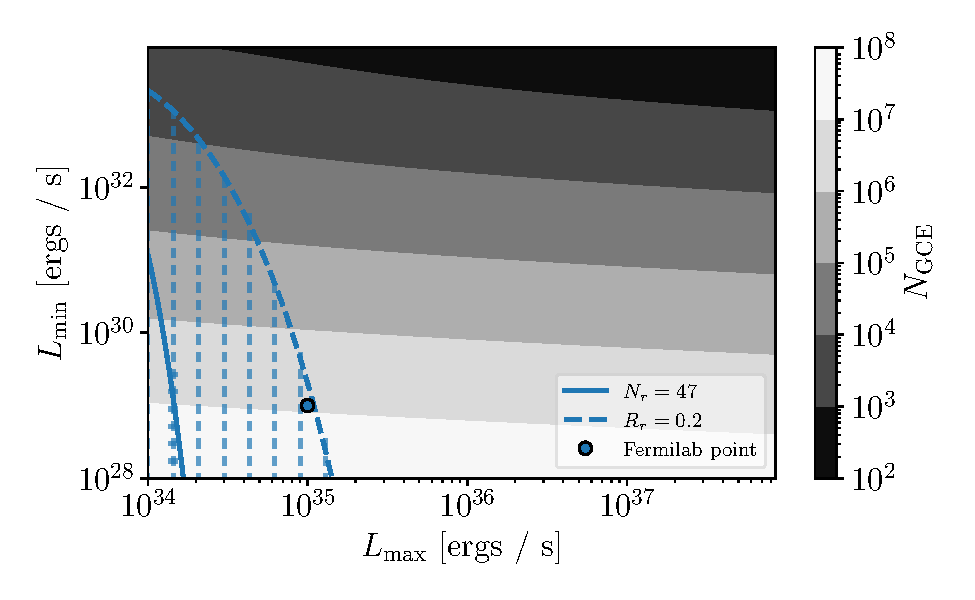
\includegraphics[width=\textwidth]{figs/power-law-step.pdf}
        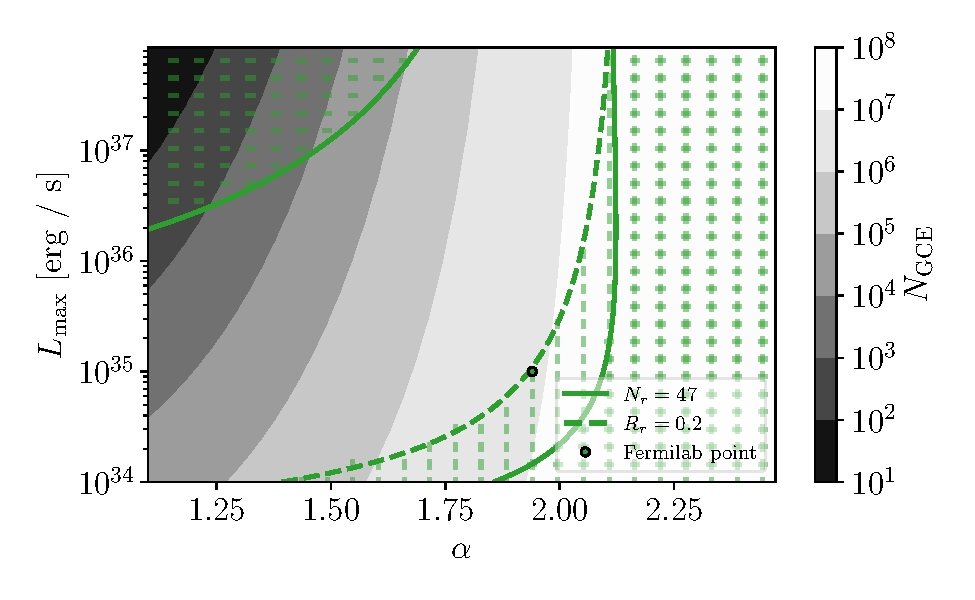
\includegraphics[width=\textwidth]{figs/power-law-alpha-step.pdf}
        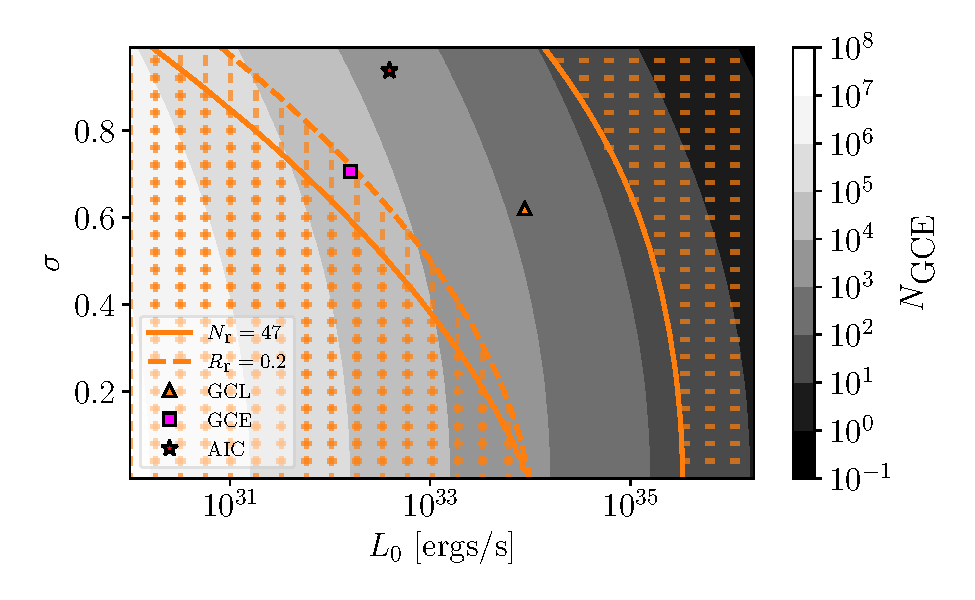
\includegraphics[width=\textwidth]{figs/log-normal-step.pdf}
        \caption{Step function sensitivity model}
        \label{fig:step-function}
    \end{subfigure}
    \hfill
    \begin{subfigure}[b]{0.49\textwidth}
        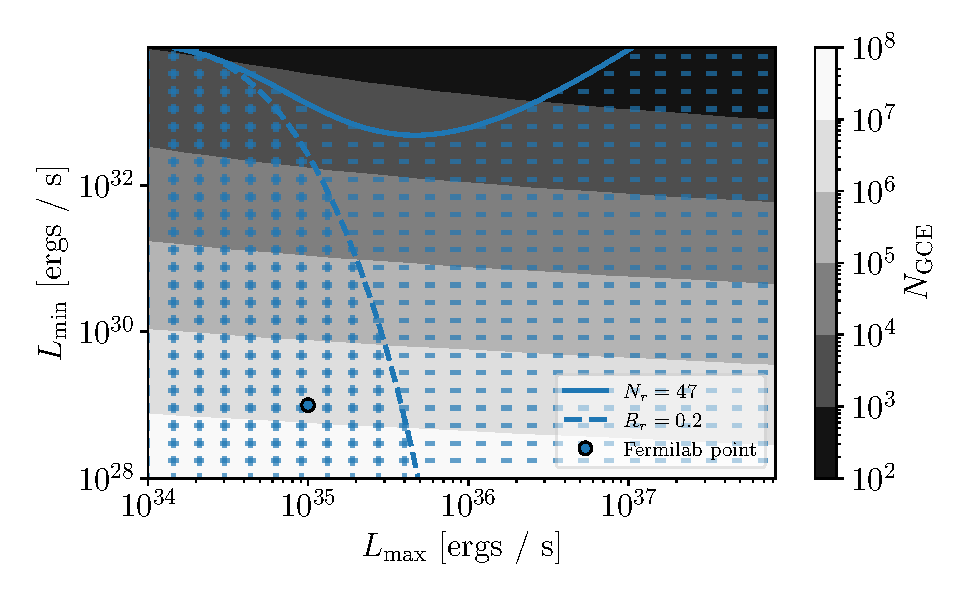
\includegraphics[width=\textwidth]{figs/power-law-pos-1x.pdf}
        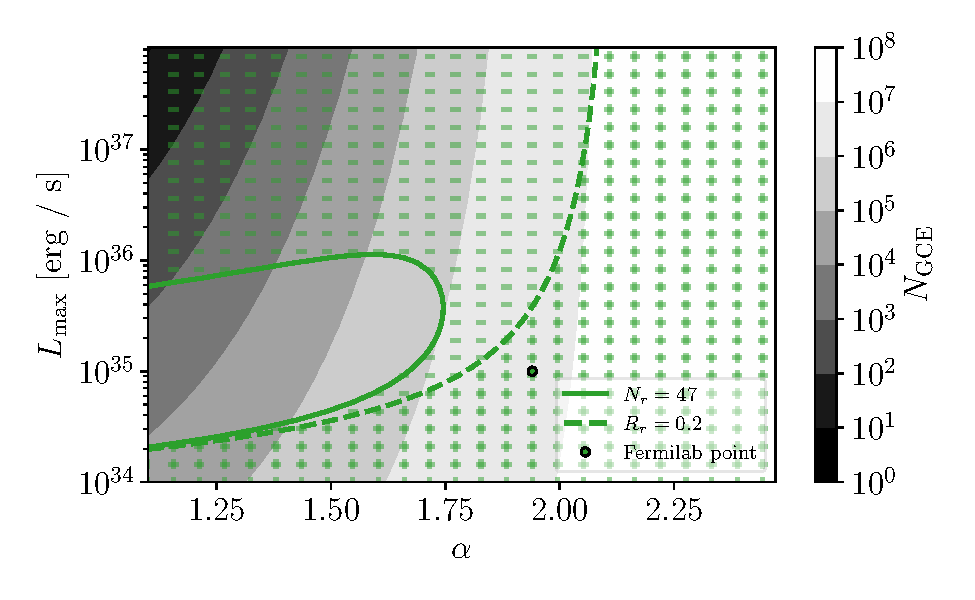
\includegraphics[width=\textwidth]{figs/power-law-alpha-pos-1x.pdf}
        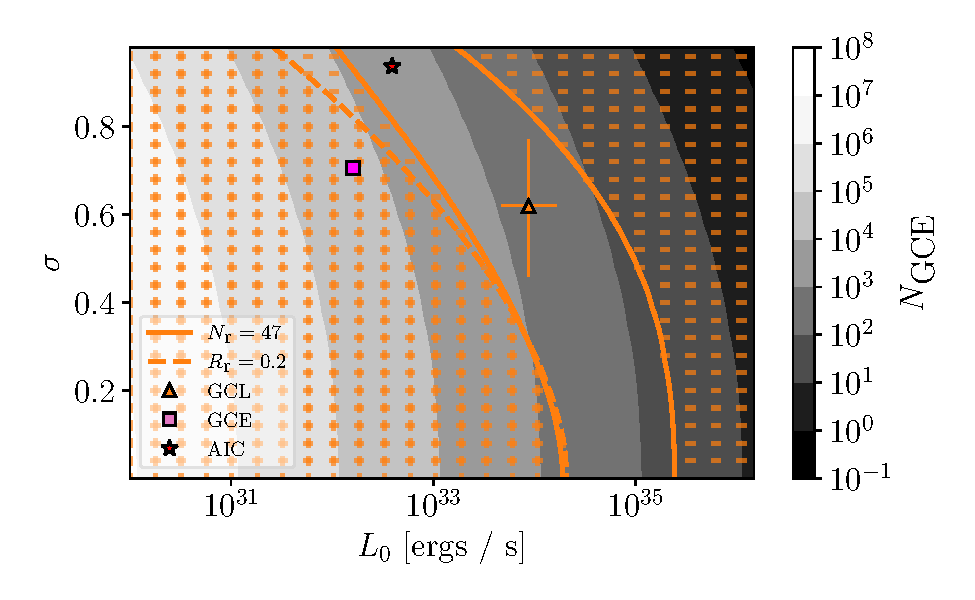
\includegraphics[width=\textwidth]{figs/log-normal-pos-1x.pdf}
        \caption{Position dependent sensitivity model}
        \label{fig:position-dependent}
    \end{subfigure}
    \caption{$N_\text{r}$, $R_\text{r}$, and $N_\text{GCE}$ calculations generated for parameterizations of a power law luminosity function (top two plots) and log normal (bottom plots). The parameterizations used in other analyses are marked. Regions allowed by the $N_\text{r} \leq 47$ and $R_\text{r} \leq 0.2$ are marked with \texttt{|} and \texttt{-} respectively, while regions allowed by both constraints are marked with \texttt{+}. The top power law plot (blue) fixes $\alpha=1.94$ while the lower (green) fixes $L_\text{min}=\SI{1e29}{erg\per\second}$ }
\end{figure}

Also shaded in these figures is the ``allowed region'' for each luminosity function---that is, the set of parameters that yield $N_\text{r} \leq 47$ and $R_\text{r} \leq 0.2$.

The analysis is also performed on the NPTF luminosity function, but only for the parameterization outlined in ref. \cite{Lee:2015fea} and therefore no figure is generated. Predictions for $N_\text{r}$, $R_\text{r}$, and $N_\text{GCE}$ for the specific parameterizations suggested by previous works are shown in tables \ref{tab:step-function-results} and \ref{tab:position-dependent-results}.

\begin{table}
    \centering
    \begin{subtable}[h]{0.55\textwidth}
        \begin{tabular}{|l|c|c|c|}
            \hline
            Luminosity function & $N_\text{r}$ & $R_\text{r}$ & $N_\text{GCE}$\\ \hline \hline
            Observation & 47 & 0.2 & \\ \hline
            Power law & 115 & 0.193 & $\num{8.14e6}$ \\
            Log normal, GCL & 296 & 0.910 & 638 \\
            Log normal, GCE & 142 & 0.180 & $\num{2.58e4}$ \\
            Log normal, AIC & 258 & 0.744 & $\num{3.87e3}$ \\
            NFW NPTF & 19.9 & 0.0136 & $\num{2.71e3}$ \\
            DISK NPTF & 208 & 0.883 & $\num{2.73e4}$ \\
            \hline
        \end{tabular}
        \caption{Step function sensitivity model}
        \label{tab:step-function-results}
    \end{subtable}
    \hfill
    \begin{subtable}[h]{0.44\textwidth}
        \begin{tabular}{|c|c|c|}
            \hline
            $N_\text{r}$ & $R_\text{r}$ & $N_\text{GCE}$\\ \hline \hline
            47 & 0.2 & \\ \hline
            17.6 & 0.101 & $\num{5.91e6}$ \\
            77.5 & 0.692 & 463 \\
            13.4 & 0.0648 & $\num{1.91e4}$ \\
            0 & 0 & $\num{0}$ \\
            7.48 & 0.0300 & $\num{1.97e3}$ \\
            71.7 & 0.757 & $\num{1.98e4}$ \\
            \hline
        \end{tabular}
        \caption{Position-dependent sensitivity model}
        \label{tab:position-dependent-results}
    \end{subtable}
    \caption{Number of resolved point sources, ratio of resolved flux to total flux, and total number of point sources predicted to make up the GCE based on four luminosity functions and the requirement that the point sources reproduce the entire flux of the GCE.}
\end{table}

The results of this analysis scale linearly with the flux of the GCE used. Figure \ref{fig:multiple-fluxes} shows figure \ref{tab:position-dependent-results} but with flux values from analyses other than di Mauro's represented. Note that $R_\text{r}$ does not vary because both fluxes in the ratio are scaled by the same amount. However, $N_\text{r}$ varies greatly for different GCE fluxes, especially in the power law case.

\begin{figure}
    \centering
    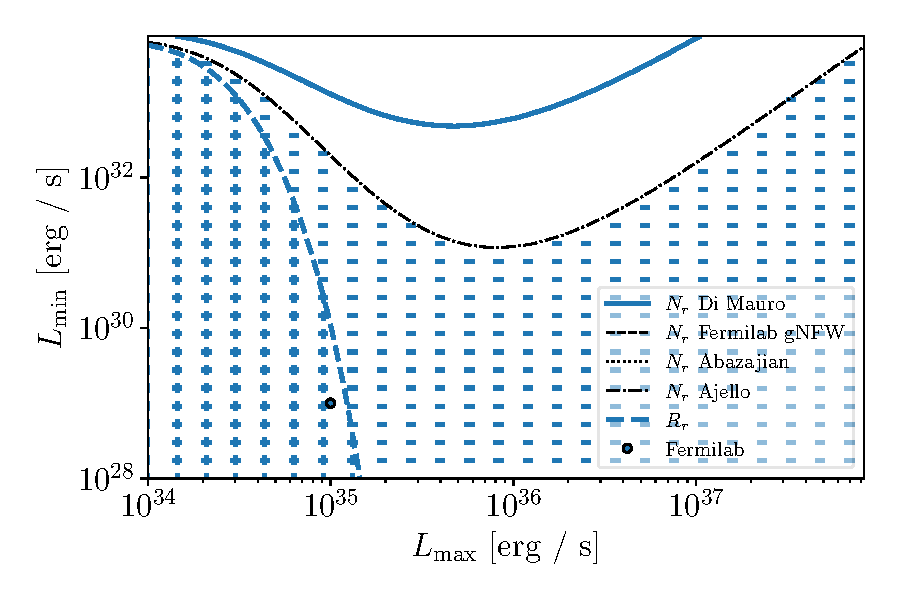
\includegraphics[width=0.49\textwidth]{figs/power-law-mult.pdf}
    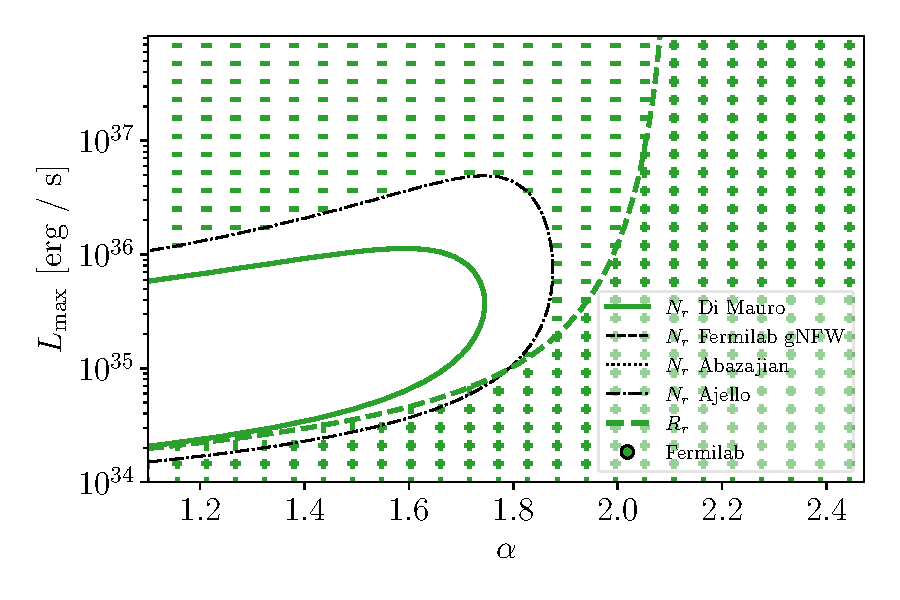
\includegraphics[width=0.49\textwidth]{figs/power-law-alpha-mult.pdf}
    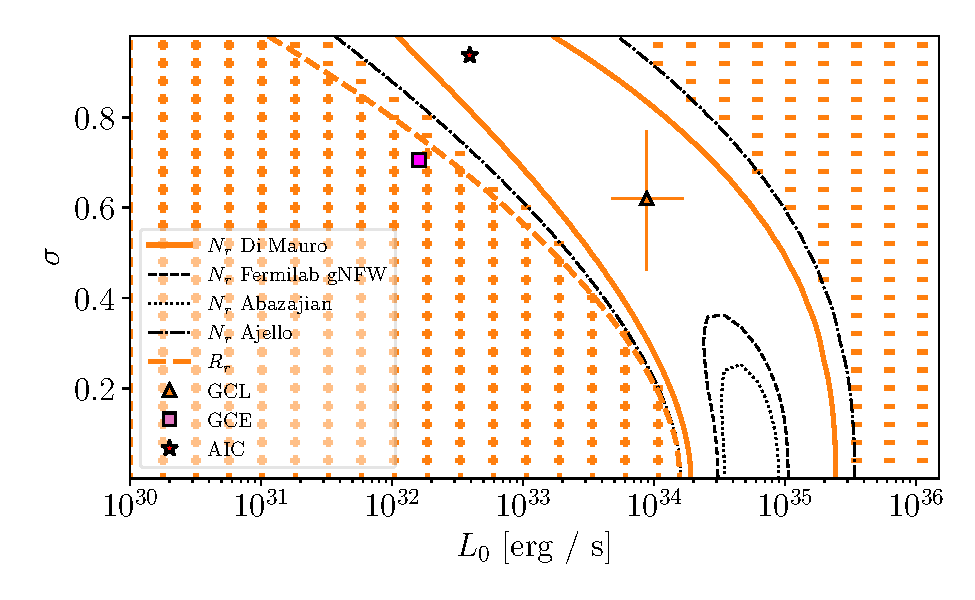
\includegraphics[width=0.49\textwidth]{figs/log-normal-mult.pdf}
    \caption{$N_\text{r}$ and $R_\text{r}$ for each luminosity function, with results for $N_\text{r}=47$ constraint shown for Fermilab gNFW's, Abazajian's, and Ajello's estimates of the GCE spectrum.}
    \label{fig:multiple-fluxes}
\end{figure}

\comment{It would probably be nice to have a table showing $N_\text{r}$ and $N_\text{GCE}$ as well.}




\subsection{Smoothed sensitivity model}

\subsection{Flux distribution}
Until this point, we have compared predictions for the population of point source in the GC to observations only through the number and flux of resolved point sources. We may expand this analysis by comparing the flux distribution of point source population as well.

Figure \ref{fig:flux-distro-fix-count} shows the flux distribution of the four luminosity functions with the number of resolvable point sources fixed at 47, which is the number we observed. The distributions are superimposed on the observed flux distribution of the 47 sources as obtained from the 4FGL catalog \cite{Fermi-LAT:2019yla}, as well as the flux distribution with the 0.53$^\circ$ cut (see section \ref{sec:observables}). Figure \ref{fig:flux-distro-fix-flux} requires each model to reproduce the total flux of the GCE, allowing the aggregate number of resolved point sources to vary. These histograms are calculated with the position-dependent sensitivity model.

\begin{figure}
    \centering
    \begin{subfigure}[b]{0.47\textwidth}
        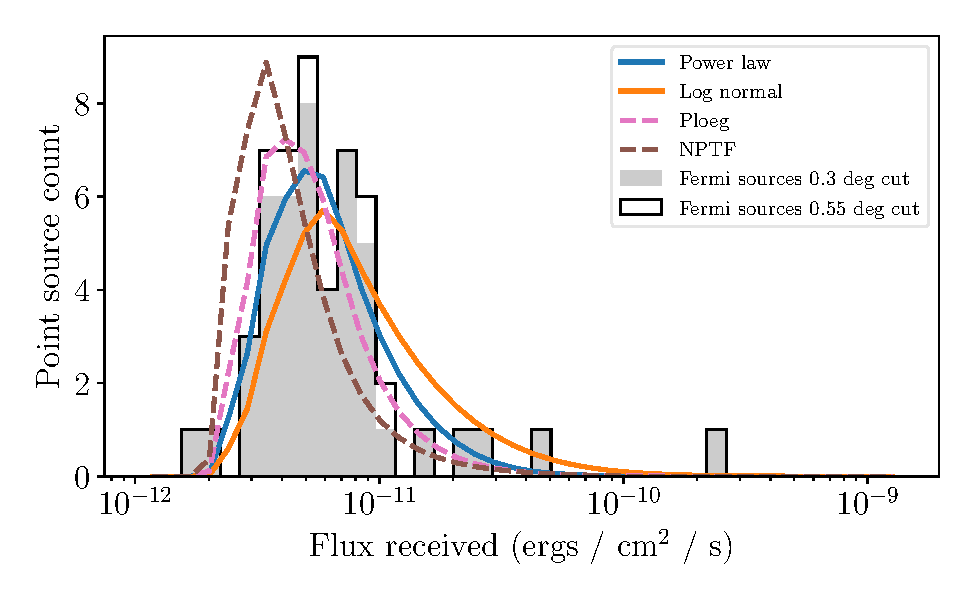
\includegraphics[width=\textwidth]{figs/flux-distro-fix-count.pdf}
        \caption{Each luminosity function is forced to reproduce 47 sources, which is the observed number}
        \label{fig:flux-distro-fix-count}
    \end{subfigure}
    \hfill
    \begin{subfigure}[b]{0.47\textwidth}
        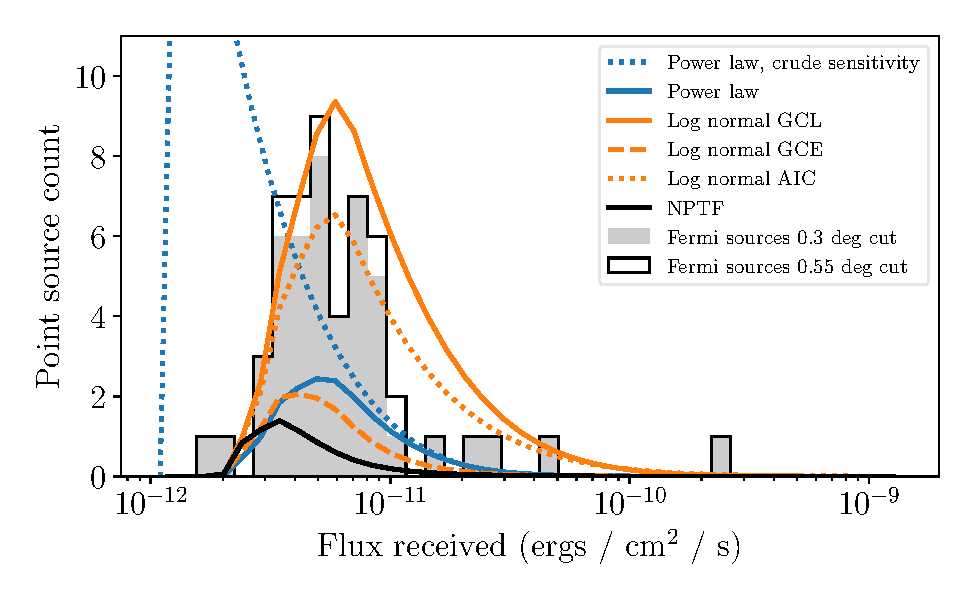
\includegraphics[width=\textwidth]{figs/flux-distro-fix-flux.pdf}
        \caption{Each luminosity function is forced to reproduce the flux of the GCE}
        \label{fig:flux-distro-fix-flux}
    \end{subfigure}
    \caption{Distribution of resolved sources predicted by each luminosity function compared to observed distribution, where observed point sources are allowed to be within 0.3$^\circ$ of spatial peaks in the GCE flux (gray histogram) and 0.53$^\circ$ (black histogram).}
\end{figure}

The total GCE flux yielded by the luminosity functions shown in figure \ref{fig:flux-distro-fix-count} which are forced to reproduce the number of observed sources is shown in table \ref{tab:rescaled-gce-flux}.

\begin{table}
    \centering
    \begin{tabular} {|l|c|c|}
        \hline
        Luminosity function & $F_\text{GCE}^\text{hyp}\ (\SI{}{\erg\per\second})$ & $F^\text{hyp}_\text{GCE} / F^\text{obs}_\text{GCE}$\\ \hline \hline
        Power law & $\num{3.49e-09}$ & $\num{2.69}$\\
        Log normal GCL & $\num{7.91e-10}$ & $\num{0.61}$ \\
        Log normal GCE & $\num{4.66e-09}$ & $\num{3.60}$\\
        Log normal AIC & $\num{0}$ & $\num{0}$ \\
        NPTF & $\num{8.29e-09}$ & $\num{6.40}$\\
        \hline
    \end{tabular}
    \caption{Total GCE flux ($F_\text{GCE}^\text{hyp}$) required by each luminosity function to yield 47 observed forces, and the ratio of that flux to the observed GCE flux $F_\text{GCE}^\text{obs}$ for comparison.}
    \label{tab:rescaled-gce-flux}
\end{table}



\section{Future Sensitivity}
We simulate an increase in sensitivity of GCE measurements by reusing the same $F_\text{th}(b, \ell)$ sensitivity map (figure \ref{fig:sensitivity}) as the one provided by the Fermi-LAT team, but with an overall multiplicative decrease. In particular, we study cases where the sensitivity is decreased by a factor of two, five, and ten and reproduce the analysis found earlier in the paper. Plots of $N_\text{r}$ for different parameterizations of the power law and log normal luminosity functions are given in figure \ref{fig:sensitivity-plots}, and values for $N_\text{r}$, $R_\text{r}$, and $N_\text{GCE}$ for specific parameterizations are given in table \ref{tab:sensitivity-values}. Of course, the number of sources in the GCE does not depend on \textit{Fermi} sensitivity and will not change. \comment{That means that the backgrounds of the column plots do not change from plot to plot. I could put them all on the same thing.}

\begin{figure}
\centering
    \begin{subfigure}[h]{0.32\textwidth}
        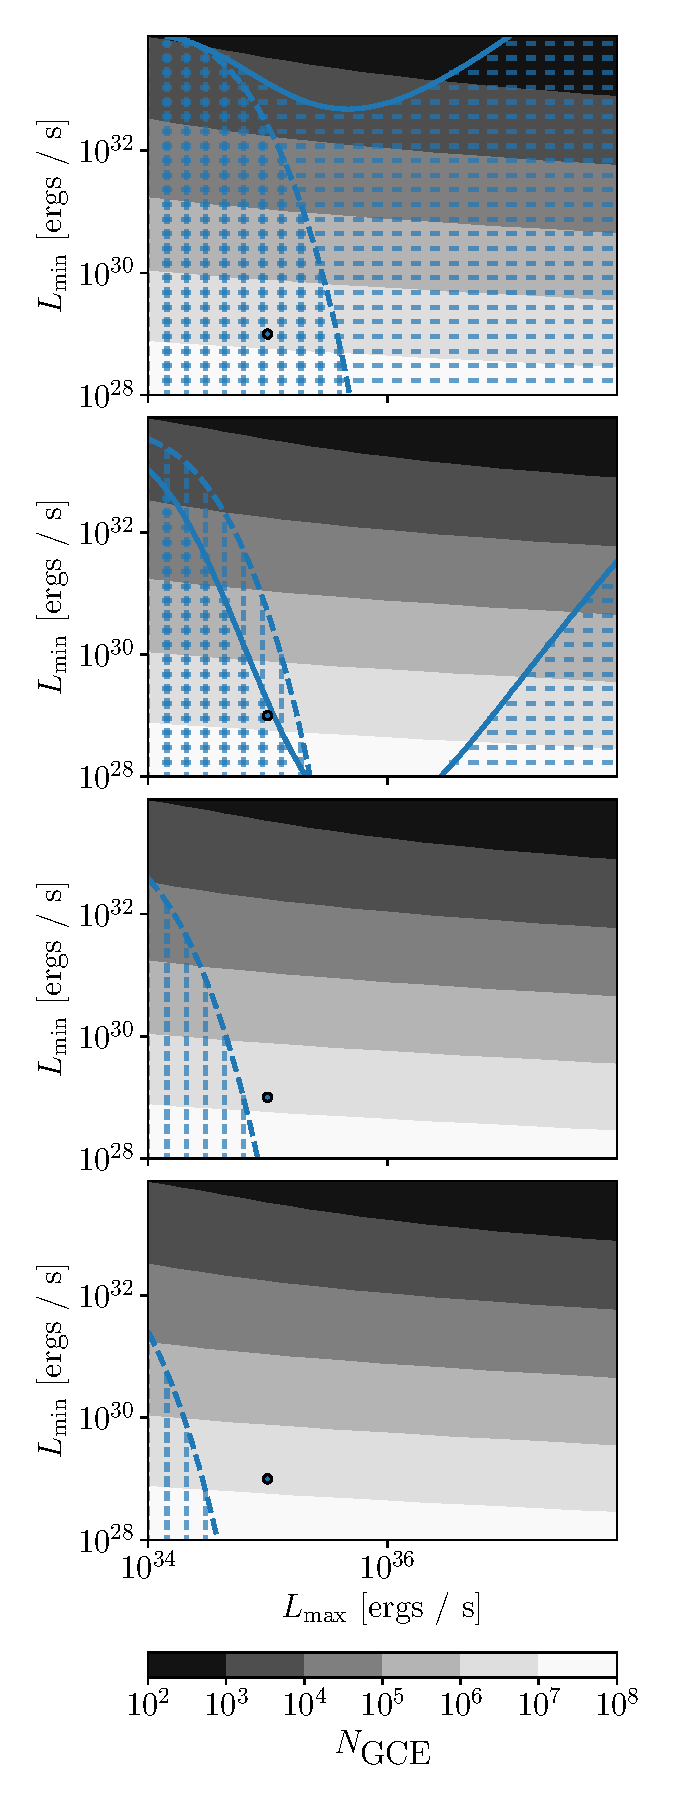
\includegraphics[width=\textwidth]{figs/power-law-sensitivity.pdf}
        \caption{Power law}
        \label{fig:sens-power-law}
    \end{subfigure}
    \hfill
    \begin{subfigure}[h]{0.32\textwidth}
        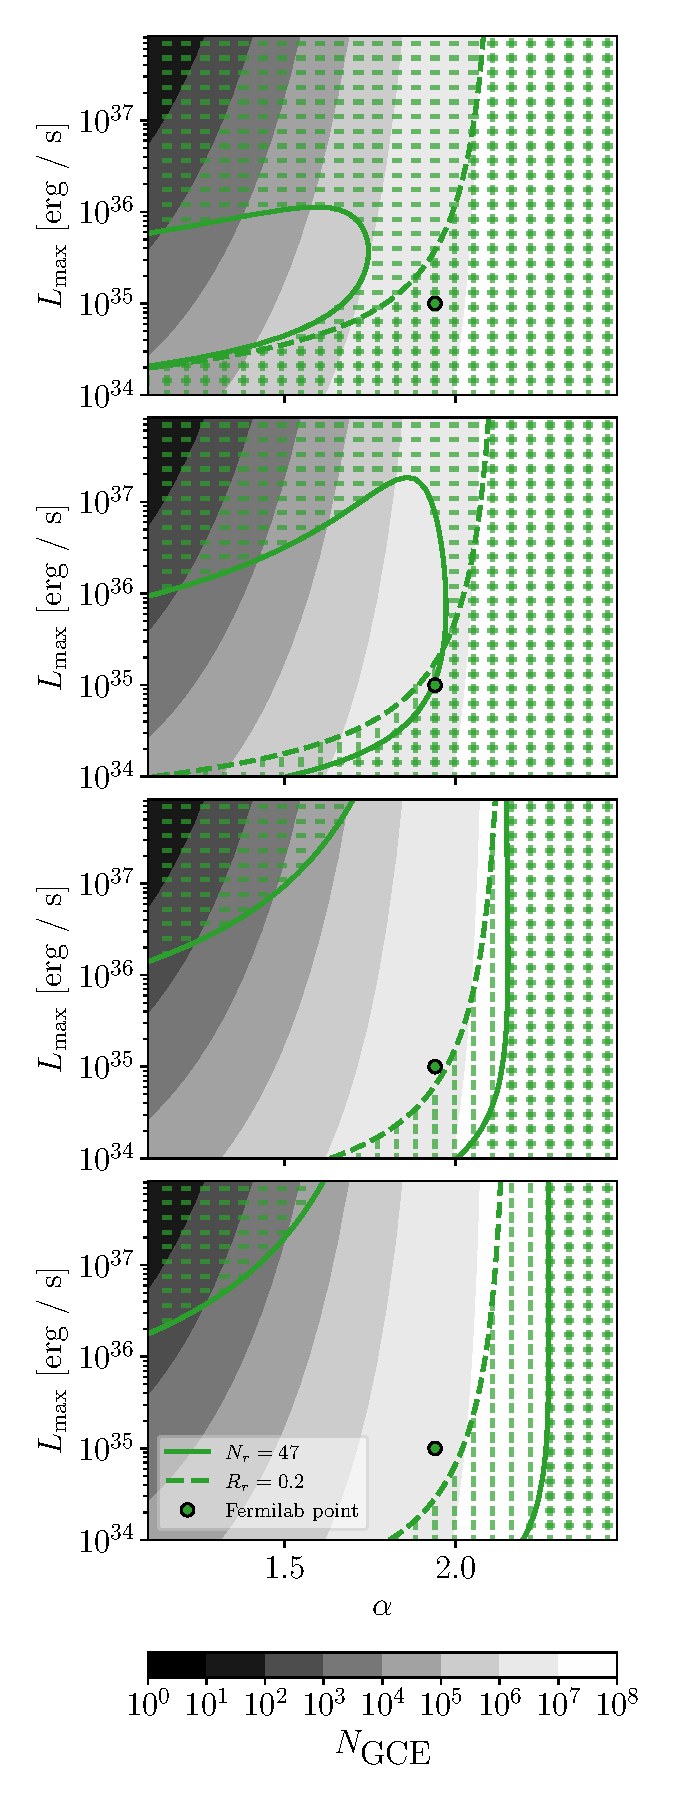
\includegraphics[width=\textwidth]{figs/power-law-alpha-sensitivity.pdf}
        \caption{Power law alpha}
        \label{fig:sens-power-law-alpha}
    \end{subfigure}
    \hfill
    \begin{subfigure}[h]{0.32\textwidth}
        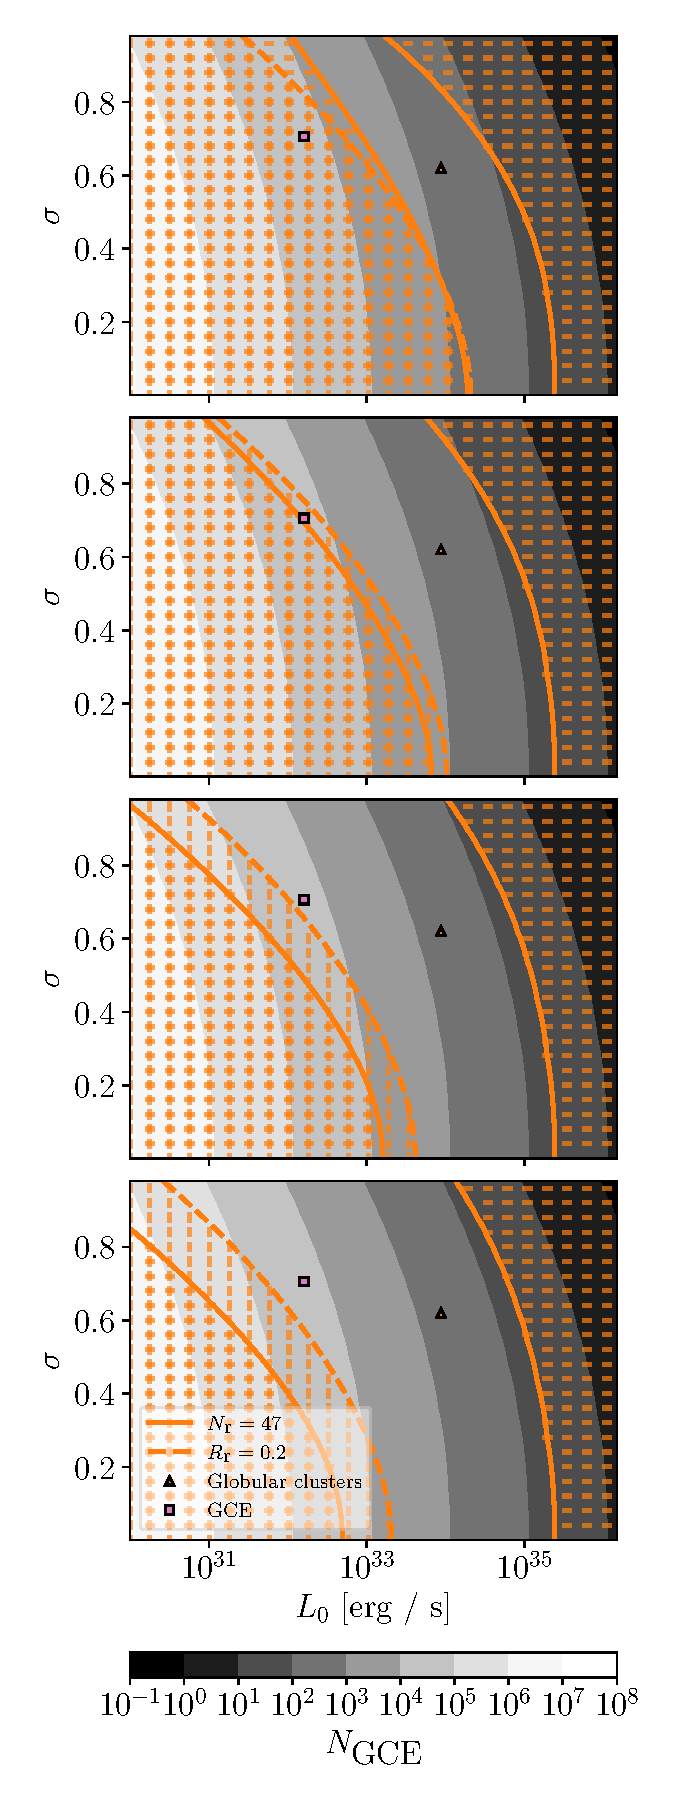
\includegraphics[width=\textwidth]{figs/log-normal-sensitivity.pdf}
        \caption{Log normal}
        \label{fig:sens-log-normal}
    \end{subfigure}
    \caption{$N_\text{r}$, $R_\text{r}$, and $N_\text{GCE}$ calculations generated for parameterizations of a power law luminosity function (left two plots) and log normal (bottom plots), for a position-dependent sensitivity model. The top three plots correspond to the current sensitivity of the \textit{Fermi} telescope (the same as figure \ref{fig:position-dependent}), while the second row assumes that the flux threshold $F_\text{th}(b, \ell)$ has been reduced by a factor of two at all points in the region of interest. The third row assumes a five times decrease and the second row assumes a ten times decrease.}
    \label{fig:sensitivity-plots}
\end{figure}

\begin{table}
    \centering
    \begin{tabular}{|l|c|c|}
        \hline
        Luminosity function & $N_\text{r}$ & $R_\text{r}$\\ \hline \hline
        Observation & 47 & \\ \hline
        Power law & 115 & $\num{8.14e6}$ \\
        Log normal, GCL & 0.910 & 638 \\
        Log normal, GCE & 0.180 & $\num{2.58e4}$ \\
        NFW NPTF & 19.9 & $\num{2.71e3}$ \\
        DISK NPTF & 208 & $\num{2.73e4}$ \\
        \hline \hline
        Power law & 115 & $\num{8.14e6}$ \\
        Log normal, GCL & 0.910 & 638 \\
        Log normal, GCE & 0.180 & $\num{2.58e4}$ \\
        NFW NPTF & 19.9 & $\num{2.71e3}$ \\
        DISK NPTF & 208 & $\num{2.73e4}$ \\
        \hline \hline
        Power law & 115 & $\num{8.14e6}$ \\
        Log normal, GCL & 0.910 & 638 \\
        Log normal, GCE & 0.180 & $\num{2.58e4}$ \\
        NFW NPTF & 19.9 & $\num{2.71e3}$ \\
        DISK NPTF & 208 & $\num{2.73e4}$ \\
        \hline \hline
        Power law & 115 & $\num{8.14e6}$ \\
        Log normal, GCL & 0.910 & 638 \\
        Log normal, GCE & 0.180 & $\num{2.58e4}$ \\
        NFW NPTF & 19.9 & $\num{2.71e3}$ \\
        DISK NPTF & 208 & $\num{2.73e4}$ \\
        \hline
    \end{tabular}
    \caption{Number of resolved point sources and total number of point sources predicted to make up the GCE based on four luminosity functions and the requirement that the point sources reproduce the entire flux of the GCE. The top row indicates the current \textit{Fermi} sensitivity, the second a twofold increase in $F_\text{th}(b, \ell)$, the third a fivefold increase, and the last a tenfold increase.}
    \label{tab:sensitivity-values}
\end{table}


\section{Conclusion}



\appendix
\section{Scaling of ROIs}
\label{sec:scale-rois}
To establish a value for the total flux of the GCE, we draw on several analyses of the GCE spectrum in section \ref{sec:total-lum}. However, not all the analyses we study use the same ROI as ours. To convert between our ROI and others', we assume an NFW squared spacial distribution of MSPs in the GCE as discussed in section \ref{sec:spacial-distro}. Then we simply calculate the ratio of flux in our region of interest $F_\Omega$ to flux in another analysis's region of interest $F_{\Omega'}$ via
\begin{equation}
    \frac{F_{\Omega'}}{F_\Omega} = \brackets{\int_{\Omega'}d\Omega\int_0^\infty ds \rho_\text{NFW}^2 (r)}\brackets{\int_{\Omega}d\Omega\int_0^\infty ds \rho_\text{NFW}^2 (r)}^{-1}.
    \label{eqn:roi-conversion}
\end{equation}
Here, $s$ represents the distance between Earth and the point of integration, and $r$ represents the galactocentric distance. They are related by $r^2 = s^2 + r_c^2 - 2 s r_c \cos\ell$, where $\ell$ is the Galactic longitude and $r_c$ is the distance between Earth and the center of the Galaxy, taken here to be $\SI{8.5}{\kilo\parsec}$ to be consistent with the rest of this study.

The flux ratio as computed by equation \ref{eqn:roi-conversion} between our region and the same $40^\circ \times 40^\circ$ without the Galactic disk cutout is 2.10. Similarly, the ratio is 1.64, 1.27, 0.915, and 1.013 \comment{Wrong!} for a $30^\circ \times 30^\circ $, $20^\circ \times 20^\circ$, $10^\circ \times 10^\circ$, and $7^\circ \times 7^\circ$ respectively.


\section{Conversion Between GCE Luminosity and Flux}
\label{app:lum-to-flux}
This analysis requires luminosity functions to be expressed as probability distributions as a function of luminosity, since they are intended to be statements solely about the GC MSP population, made without reference to the distance of observation, and therefore the flux. Yet several papers referenced in this study express luminosity functions as a function of flux. This appendix describes how the conversion to luminosity is done.

As discussed in section \ref{sec:spacial-distro}, we represent the MSP population as distributed according to an NFW squared distribution with $\gamma = 1.2$. One way to convert a function of flux to luminosity would be to simply use the luminosity function which, when integrated over the NFW squared spacial distribution, would reproduce the observed function of flux. But this method would change the functional form of the luminosity function so that, for example, a luminosity function that is log normal when written in terms of flux would no longer be log normal when written in terms of luminosity. \comment{Is it worth devoting a whole paragraph to describing something I do not intend to do? I do it to avoid confusion.}

So for this paper, we simply convert the flux value of every bin to a luminosity according to the following method. We assume that the entire population of MPSs only contains pulsars with luminosity $L$ and ask what average flux $F$ per pulsar is observed. Integrated over the region of interest $\Omega$, this yields a constant flux to luminosity ratio of
\begin{equation}
    \frac{F}{L} = \frac{1}{4\pi}\brackets{\int_{\Omega}d\Omega\int_0^\infty ds \rho_\text{NFW}^2 (r)}\brackets{\int_{\Omega}d\Omega \int_0^\infty s^2 ds \rho_\text{NFW}^2 (r)}^{-1} = \SI{1.11e-46}{\per\centi\meter\squared}.
    \label{eqn:f-to-l}
\end{equation}
Here, $s$ represents the distance from Earth to the point of integration, and $r$ represents the distance from the GC to the point of integration. They are related by the law of cosines: $r^2 = s^2 + r_c^2 - 2s r_c \cos \ell$, where $\ell$ is the Galactic longitude. The numerical value reported was computed for $r_c = \SI{8.5}{\kilo\parsec}$. It is slightly lower than the na\"ive value of $\frac{F}{L} = \frac{1}{4\pi r_c^2} = \SI{1.16e-46}{\per\centi\meter\squared}$, which assumes that all the MSPs are at the Galactic center, and therefore does not rely on a choice of $\gamma$.


\section{Calculation of photon energy}
\label{app:photon-energy}
The parameterization of the NPTF luminosity function of ref. \cite{Lee:2015fea} is given with flux units of photons per second. To convert this to luminosity via appendix \ref{app:lum-to-flux}, we need to find the energy of a single GCE photon. To do this, we fit a broken power law to the GCE spectrum found by di Mauro and described in section \ref{sec:total-lum}, defining the flux observed from photons in an energy bin of energy $E_\gamma$ and width $dE_\gamma$ as $dF = E_\gamma N(E_\gamma)dE_\gamma$. The function $E_\gamma N(E_\gamma)$ is plotted in figure \ref{fig:di-mauro-example}. The average photon energy is then calculated by
\begin{equation}
    \langle E_\gamma \rangle =  \brackets{\int_{\SI{0.1}{\giga\electronvolt}}^{\SI{100}{\giga\electronvolt}} E_\gamma N(E_\gamma) dE_\gamma} \brackets{\int_{\SI{0.1}{\giga\electronvolt}}^{\SI{100}{\giga\electronvolt}} N(E_\gamma) dE_\gamma}^{-1} = \SI{0}{\giga\electronvolt}.
    \label{eqn:photon-energy}
\end{equation}
\comment{I'd like to finish this. Give examples of photon energy.}



\acknowledgments

This is the most common positions for acknowledgments. A macro is
available to maintain the same layout and spelling of the heading.






% The bibliography will probably be heavily edited during typesetting.
% We'll parse it and, using the arxiv number or the journal data, will
% query inspire, trying to verify the data (this will probalby spot
% eventual typos) and retrive the document DOI and eventual errata.
% We however suggest to always provide author, title and journal data:
% in short all the informations that clearly identify a document.


\bibliographystyle{plain}
\bibliography{gce.bib}

\end{document}
